\documentclass[11pt]{article}
\usepackage{setspace}
\setstretch{1}
\usepackage{amsmath,amssymb, amsthm}
\usepackage{graphicx}
\usepackage{bm}
\usepackage[hang, flushmargin]{footmisc}
\usepackage[colorlinks=true]{hyperref}
\usepackage[nameinlink]{cleveref}
\usepackage{footnotebackref}
\usepackage{url}
\usepackage{listings}
\usepackage[most]{tcolorbox}
\usepackage{inconsolata}
\usepackage[papersize={8.5in,11in}, margin=1in]{geometry}
\usepackage{float}
\usepackage{caption}
\usepackage{esint}
\usepackage{url}
\usepackage{enumitem}
\usepackage{subfig}
\usepackage{wasysym}
\newcommand{\ilc}{\texttt}
\newcommand{\p}{\partial}
\usepackage{etoolbox}
\usepackage{algorithm}
\usepackage{changepage}
% \usepackage{algorithmic}
\usepackage[noend]{algpseudocode}
\usepackage{tikz}


\usetikzlibrary{matrix,positioning,arrows.meta,arrows}
\patchcmd{\thebibliography}{\section*{\refname}}{}{}{}
% \PassOptionsToPackage{hyphens}{url}\usepackage{hyperref}

\providecommand{\myceil}[1]{\left \lceil #1 \right \rceil }
\providecommand{\myfloor}[1]{\left \lfloor #1 \right \rfloor }

\definecolor{dkgreen}{rgb}{0,0.6,0}
\definecolor{gray}{rgb}{0.5,0.5,0.5}
\definecolor{mauve}{rgb}{0.58,0,0.82}

\lstset{frame=tb,
  language=Python,
  aboveskip=3mm,
  belowskip=3mm,
  showstringspaces=false,
  columns=flexible,
  basicstyle={\small\ttfamily},
  numbers=none,
  numberstyle=\tiny\color{gray},
  keywordstyle=\color{blue},
  commentstyle=\color{dkgreen},
  stringstyle=\color{mauve},
  breaklines=true,
  breakatwhitespace=true,
  tabsize=3
}

\begin{document}


\title{\textbf{CSDS 491: Assignment 2}}

\author{Shaochen (Henry) ZHONG, \ilc{sxz517@case.edu}}

\date{Due and submitted on 03/08/2021 \\ Spring 2021, Dr. Lewicki}
\maketitle


% We've received some common questions for A1.  Here are some hints to help you go in the right direction.
%
% Q2.2: You need only prove there is a logical gap that would require an additional assumption.
%
% Q4: It is helpful to use the conjugate prior as shown in lecture.  The  normalization factor for the posterior then has the same form as the prior (but with different arguments).
%
% Q5: Remember that the data consists of event times, and the posterior is in terms of the Poisson rate parameter lambda given the number of observed data events in a given duration from 0 to T.  You only need a single Poisson likelihood combined with the prior to get the posterior.
%
% Exploration: The terms discrete and continuous refer to the variables in the model.  See the rubric for the grading criteria. Try to make your inference problems simple models of real-world situations, rather than just numerical examples.


\section*{Q1. Conditional Independence}

\subsection*{1.1.}

\begin{align*}
    p(a,b) &= \sum\limits_c \sum\limits_d \sum\limits_e p(a, b, c, d, e) \\
    &= \sum\limits_c  p(c \mid a, b) p(a)p(b) \cdot \sum\limits_d p(d \mid c) \cdot \sum\limits_e p(e \mid c) \\
    &\text{Known that} \ \sum\limits_{x} p(x \mid pa(x)) = 1 \\
    &= p(a)p(b)
\end{align*}

Thus, $a \perp b \mid \emptyset$.

\subsection*{1.2.}

For $a \perp b \mid e$ we must have $p(a, b \mid e) = p(a \mid e) p(b \mid e)$. Which implies $p(a \mid b, e) = p(a \mid e)$ since:

\begin{align*}
    p(a \mid b) &= \frac{p(a, b)}{p(b)} \\
    p(a \mid b, e) &= \frac{p(a, b \mid e)}{p(b \mid e)} \\
    &= \frac{p(a \mid e) p(b \mid e)}{p(b \mid e)} \\
    &= p(a \mid e)
\end{align*}

Known that $a \perp b \mid \emptyset$, now to calculate $p(a \mid b, e)$ and $p(a \mid e)$ to see if they are equal:

\begin{align*}
    p(a \mid b,e) &= \frac{p(a,b,e)}{p(b,e)} = \frac{\sum_c p(a,b,c,e)}{\sum_a\sum_c p(a,b,c,e)}\\
    &= \frac{\sum_c p(e \mid c)p(a,b,c)}{\sum_a\sum_c p(e \mid c)p(a,b,c)}\\
    &= \frac{\sum_c p(e \mid c)p(a,b,c)}{\sum_a\sum_c p(e \mid c)p(c \mid a, b) p(a, b)}\\
    &= \frac{\sum_c p(e \mid c)p(a,b,c)}{\sum_a\sum_c p(e \mid c)p(c \mid a, b) p(a) p(b)}\\
    &= \frac{\sum_c p(e \mid c)p(a,b,c)}{\sum_c p(e \mid c)p(b, c)}
\end{align*}

\begin{align*}
    p(a \mid e) &= \frac{p(a,e)}{p(e)} = \frac{\sum_c\sum_b p(a,b,c,e)}{\sum_c p(e \mid c)p(c)}\\
    &= \frac{\sum_c p(e \mid c) \sum_b p(a,b,c)}{\sum_c p(e \mid c)p(c)}\\
    &= \frac{\sum_c p(e \mid c) p(a,c)}{\sum_c p(e \mid c)p(c)}
\end{align*}


Thus, it is possible that $p(a \mid b,e) \neq p(a \mid e)$ unless we may confirm that $p(b) = 1$.


\section*{Q2. Conditional Independence and Causality}

The conditional independence assumption this model made is $b \perp c \mid a$ as $p(b, c \mid a) = p(b \mid a) p(c \mid a)$; and joint distribution of this model is therefore $p(a, b, c) = p(b\mid  a)p(c\mid a)p(a)$.

However, the same joint distribution $p(a, b, c)$ can also be modeled differently:

\begin{align*}
    p(a, b, c) &= p(a \mid b, c)p(b \mid c)p(c) \\
    &= p(b \mid a, c)p(a \mid c)p(c) \\
    &= p(c \mid a, b)p(a \mid b)p(b) \\
    &= \dots
\end{align*}

Thus, the condition of the purposed graph does not necessarily hold.


\section*{Q3. Model Complexity, Free Parameters, and Simplifying Assumptions}

\subsection*{3.1.}

\begin{align*}
    p(x_1, x_2, \dots, x_N) &= p(x_1 \mid x_2, x_3, \dots, x_N) p(x_2, x_3, \dots, x_N) \\
    &= p(x_1 \mid x_2, x_3, \dots, x_N) p(x_2 \mid x_3, x_4, \dots, x_N) p(x_3, \dots, x_N) \\
    &= p(x_N) \cdot \prod_{i = 1}^{N-1} p(x_i \mid x_{i+1},  x_{i+2}, \dots, x_{N})
\end{align*}

\subsection*{3.2.}

This questions is essentially asking how many combination can we have for $\{ x_1, x_2, \dots, x_N \}$ given each $x_i$ has $K$ differrents states. As there will be $K^N$ combinations, there will be $K^N - 1$ parameters needed since the last state of the last node will not need another new parameter (it can be represent as the negation of all other states).

Similarily, we may continue upon the formula obtained in above question where $p(x_N) \cdot \prod_{i = 1}^{N-1} p(x_i \mid x_{i+1},  x_{i+2}, \dots, x_{N})$. Known that $x_N$ needs $(K-1)$ parameters to represent (since the last state can be represent as the negation of all other states) and a node with $i$ parents need $K^i$ parameters to represent.

\begin{align*}
    \sum_{i = 1}^{N} (K-1)(K^{N - i}) &= (K - 1)(K^{N - 1}) + (K - 1)(K^{N - 2}) + \dots + (K - 1)(K^0) \\
    &= (K-1) \cdot \frac{K^N - 1}{K - 1} = K^N - 1
\end{align*}

And $K^N - 1$ will be generalized as $O(K^N)$.

\subsection*{3.3.}

The $m$ root nodes each with $K$ stats will need $m(K - 1)$ parameters. The $N-m$ leaf nodes will each have $(K-1)$ parameters needed for itself and $K^m$ parameters needed for its $m$ of $K$-state parents. Thus, we will have:

\begin{equation*}
    m(K - 1 ) + (N-m)(K-1)K^m
\end{equation*}

parameters needed.

\subsection*{3.4.}

Since the formula of noisy-OR is given in a ``leaky'' fashion $p(x_i \mid \textrm{pa}({x_i})) = 1 - (1 - \mu_{i0}) \prod_{j \in \textrm{pa}(x_i)}(1 - \mu_{ij})^{x_j}$ where a $(1 - \mu_{i0})$ is involved. Each leaf nodes will have $(K-1)$ parameters needed for itself, and each of its parents will need $m^(k-1)$ parameters as each parent node has $k$ states (but since we only need a single parent at a time so we don't need another new parameter for the last state, so $k-1$). Last, we need one more parameter for the leak node $\mu_{i0}$ for each leaf node. All others remain unchanged and we have (note $K - 1 = 1$):

\begin{equation*}
    m(K-1) + (N-m)(K-1)(m^{K-1} + 1)= m + (N-m)(m + 1)
\end{equation*}

\section*{Q4. Models of Conditional Probability}


\subsection*{4.1.}

There must be at least a parent $x_j = 1$ as otherwise for $p(x_i = 1 \mid \textrm{pa}(x_i)) = 1 - (1 - \mu_{i0}) \cdot \prod_{j \in \textrm{pa}(x_i)} (1 - \mu_{ij})^0 = 1 - 1(1 - \mu_{i0})$ which will be very close to $0$; in fact, $p(x_i = 1 \mid \textrm{pa}(x_i))$ will be $0$ if we don't consider the leak node. So we know that there must be at least $x_j = 1$.\newline

This means if we have one $x_j = 1$ with a high $\mu_{ij} = \p(x_i = 1 \mid x_j = 1)$, we will have a very low $1 - \mu_{ij}$ and therefore bring the overall $p(x_i = 1 \mid \textrm{pa}(x_i))$ to be closer to zero. Since only one $x_i = x_j = 1$ with a high $\mu_{ij}$ will dramatically increase the overall output of  $p(x_i = 1 \mid \textrm{pa}(x_i))$, this works similar to the OR gate which will make $p(x_i = 1 \mid \textrm{pa}(x_i)) = 1$ with just one of its parent nodes being $1$. The noisy-OR is considered to be ``soft'' as it won't make the $p(x_i = 1 \mid \textrm{pa}(x_i))$ to be exactly 1 but only close to 1.

\subsection*{4.2.}

It is a leak node defined in the D\'{i}ez version of Leaky Noisy-OR function. It is aim to compensate the fact that in a complicate model, a $x_i$ can be 1 even if all of its parents are not 1 -- which can be roughly understand as a prior/bias base on prior knowlegde to the model.

Since we may assign a value to each $\mu_{i0}$, even if all parents of $x_i$ are zeros, we have:

\begin{align*}
    p(x_i \mid \textrm{pa}({x_i})) &= 1 - (1 - \mu_{i0}) \prod_{j \in \textrm{pa}(x_i)}(1 - \mu_{ij})^{x_j} \\
    &= 1 - (1 - \mu_{i0}) \prod_{j \in \textrm{pa}(x_i)}(1 - \mu_{ij})^0 \\
    &= \mu_{i0}
\end{align*}

Note it is only the D\'{i}ez version of leaky noisy-OR function as it was made on the assumption that the prior knowlegde will not have any effect on the output of modeled variables (the conditional output given the parents, namely all the $\mu_{ij}$s). Where Henrion considered the prior knowlegde will affect the output of all modeled variables as $p(x_i \mid \textrm{pa}({x_i})) = 1 - (1 - \mu_{i0}) \prod_{j \in \textrm{pa}(x_i)}(\frac{1 - \mu_{ij}}{1 - \mu_{i0}})^{x_j}$ where the $(1 - \mu_{i0})$ is part of every $u_{ij}$ outputs.

\subsection*{4.3.}

We may do the following transformation to the noisy-OR function and express it in a fashion of sum-of-weighted-inputs. For the ease of expression we will ignore the $1 - \mu_{i0}$ as it can be considered as a special parent and merge into to the $\prod_{j \in \{ \textrm{pa}(x_i) + x_0 \}}(1 - \mu_{ij})^{x_j}$. So we have the noisy-OR function being:

\begin{equation*}
    p(x_i \mid \textrm{pa}({x_i})) = 1 - \prod_{j \in \{ \textrm{pa}(x_i) + x_0 \}} (1 - \mu_{ij})^{x_j}
\end{equation*}

If we set $W_{ij} = - \ln(1 - \mu_{ij})$, we may express the nosiy-OR as (note for all $j$ we have $j \in \{ \textrm{pa}(x_i) + x_0 \}$):

\begin{align*}
    p(x_i \mid \textrm{pa}({x_i})) &= \rho (\sum_j W_{ij} \cdot x_{j}) \\
    \rho(z) &= 1 - e^{-z}
\end{align*}

We may confirm this is equivalent to the original noisy-OR function as:

\begin{align*}
    p(x_i \mid \textrm{pa}({x_i})) &= 1 - e^{-\sum_j W_{ij} \cdot x_{j}} \\
    &=1 - \frac{1}{e^{\sum_j -\ln(1 - \mu_{ij}) x_j}} \\
    &= 1 - \frac{1}{\prod_j \frac{1}{(1 - \mu_{ij}) ^ {x_j}}} \\
    &= 1 - \prod_j (1 - \mu_{ij})^{x_j}
\end{align*}

So essentially, we have the noisy-OR and sigmoid $\sigma(z) = \frac{1}{1 + e^{-z}} = 1 - \sigma(-z)$ both being a transformation function of a sum of weighted inputs. However, the sigmoid function is more general as is can take negative weights for $W_ij$, where for noisy-OR it can't since $W_{ij} = - \ln(1 - \mu_{ij})$. Moreover, noisy-OR can only take weights in the range of $(-\ln(0), -\ln(1)]$, where sigmoid can take any value to be its weights.

Due to the weight limitation issue, sigmoid can certainly compute unique functions where noisy-OR can't. But for model which needs extreme probablity (need $\{0, 1 \}$ as outputs), sigmoid function might not be applied due to it will need some extremely large negative/positive weights to bring the $\sigma(z)$ to 0 or 1. This can often be a problem if a model was operating base on the assumption of noisy-OR, and I will show one example in the below question where noisy-OR works but sigmoid doesn't; where the probablity output of the model is exactly like the prediction of noisy-OR.


\subsection*{4.4.}

First for a model which sigmoid works but noist-OR doesn't, the AND gate can be a perfect example where we have (where $x_{j1}, x_{j2}$ are parent nodes of $x_i$):

\begin{table}[H]
    \centering
    \begin{tabular}{ c  c | c }
        \hline
        $x_{j1}$ & $x_{j2}$ & $x_i$ \\
        \hline
        0 & 0 & 0 \\
        0 & 1 & 0 \\
        1 & 0 & 0 \\
        1 & 1 & 1
    \end{tabular}
\end{table}

To model this distribution with noisy-OR function, we have (note we ignore the leak node here to simplify the expression):

\begin{align*}
    p(x_i = 1 \mid x_{j1} = 0, x_{j2} = 0) &= 1 - (1 - p(x_i = 1 \mid x_{j1} = 0))^{0} \cdot (1 - p(x_i = 1 \mid x_{j2} = 0))^{0} = 0 \\
    p(x_i = 1 \mid x_{j1} = 0, x_{j2} = 1) &= 1 - (1 - p(x_i = 1 \mid x_{j1} = 0))^{0} \cdot (1 - p(x_i = 1 \mid x_{j2} = 1))^{1}\\ &= 1 - \frac{1}{2}= \frac{1}{2} & \text{Should be 0}\\
    p(x_i = 1 \mid x_{j1} = 1, x_{j2} = 0) &= 1 - (1 - p(x_i = 1 \mid x_{j1} = 1))^{1} \cdot (1 - p(x_i = 1 \mid x_{j2} = 0))^{0} \\ &= 1 - \frac{1}{2}= \frac{1}{2} & \text{Should be 0}\\
    p(x_i = 1 \mid x_{j1} = 1, x_{j2} = 1) &= 1 - (1 - p(x_i = 1 \mid x_{j1} = 1))^{1} \cdot (1 - p(x_i = 1 \mid x_{j2} = 1))^{1} \\ &= 1 - \frac{1}{2} \cdot \frac{1}{2}= \frac{3}{4} & \text{Should be 1}    % p(x_i = 1 \mid \textrm{pa}(x)) &= 1 - \frac{1}{2} \cdot \frac{1}{2}= \frac{3}{4} & \text{Should be $\frac{1}{4}$}
\end{align*}

As shown, the noisy-OR cannot model this system accurately, and this can't be solved by introducing a leak node -- since for the same $x_i$, the output answer has a different diffrence to the desired answer.\newline

\noindent However, if we use the sigmoid function to model this distribution, we may view the three neurons (events) as following:

\begin{figure}[H]
    \centering
    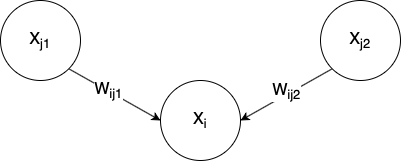
\includegraphics[width=0.6\linewidth]{{fig/p4.4}.png}
\end{figure}

And we may set $W_{ij1} = W_{ij2} = m$ and set the bias of $x_i$ to be $-1.5m$; where such $m$ must be large enough such as $\sigma(0.5m) \approx 1$. Now to calculate the probablity outputs:

\begin{align*}
    p(x_i = 1 \mid x_{j1} = 0, x_{j2} = 0) &= \sigma(0 - 1.5m) \approx 0 \\
    p(x_i = 1 \mid x_{j1} = 0, x_{j2} = 1) &= \sigma(1m - 1.5m) \approx 0 \\
    p(x_i = 1 \mid x_{j1} = 1, x_{j2} = 0) &= \sigma(1m - 1.5m) \approx 0 \\
    p(x_i = 1 \mid x_{j1} = 1, x_{j2} = 1) &=  \sigma(2m - 1.5m) \approx 1
\end{align*}

Clearly sigmoid can model this distribution as desired. This is because in sigmoid we can take an arbitrarily large weight between neurons (in this case, $m$) but we can't do such thing in noisy-OR. \newline


\noindent However, there are also distributions that can only be nicely modeled by noisy-OR but not sigmoid. Intuitively, a distribution that follows noisy-OR must be modeable by the noist-OR function; and here's an example of how a distribution follows noisy-OR assumptions can't be modeled by sigmoid.

In the above section we already established that the noisy-OR function can also be expressed as sum-of-weighted-inputs:

\begin{align*}
    p(x_i \mid \textrm{pa}({x_i})) &= \rho (\sum_j W_{ij} \cdot x_{j}) \\
    \rho(z) &= 1 - e^{-z}
\end{align*}

So if we reuse the above diagram, but set $W_{ij1} = -\ln(1 - \mu{ij1})$ and $W_{ij2} = -\ln(1 - \mu{ij2})$, we may have a distribution of:

\begin{table}[H]
    \centering
    \begin{tabular}{ c  c | c }
        \hline
        $x_{j1}$ & $x_{j2}$ & $p(x_i)$ \\
        \hline
        0 & 0 & 0 \\
        0 & 1 & $1-e^{-1}$ \\
        1 & 0 & $1-e^{-1}$ \\
        1 & 1 & $1-e^{-2}$
    \end{tabular}
\end{table}

It is trivial to show that this distribution can be modeled by the noisy-OR function as it is defined with respect to noisy-OR. So the only thing left is to show that this distribution cannot be nicely modeled by the sigmoid function.

However, this is an impossible task because:

\begin{itemize}
    \item To have $p(x_i  \mid x_{j1} = 0, x_{j2} = 0) = 0$ we must have very large and negative sum-of-weighted-inputs $z$ to bring $\sigma(z - \text{}) \approx 0$. This can be done by setting a very large and negative bias on $x_i$, like $-m$.
    \item To have $p(x_i \mid x_{j1} = 0, x_{j2} = 1), p(x_i  \mid x_{j1} = 1, x_{j2} = 0) = 1-e^{-1}$, since $1-e^{-1}$ is a positive value, we must have the $W_{ij1}, W_{ij2}$ to be greater than the absolute value of the bias $|-m|$ so that we will have $\sigma(W_{ij1} - m)$ or $\sigma(W_{ij2} - m)$ to be $\geq 0$. This means $W_{ij1}, W_{ij2}$ must be some significantly large positive value that is $> m$.
    \item Since we have established that $W_{ij1}, W_{ij2}$ must be some significantly large positive value that is $> m$. For $p(x_i \mid x_{j1} = 1, x_{j2} = 1)$ with the sigmoid function we must have $\sigma(z = W_{ij1} + W_{ij2} - m)$; where such $z$ is guaranteed to be $>m$ and we know that $\sigma(m) \approx 1$. This will create an unavoidable confict with the purposed distribution as the output should be $1-e^{-2}$ which is $\ll 1$.
\end{itemize}

So we have showed an example distribution where the noisy-OR function works but the sigmoid function doesn't. This is because to have outputs like $\{0, 1\}$ sigmoid, we must relay on large weights and large bias; but since the distribution is defined with respect to noisy-OR, it was desiged to use with smaller weights.\newline


\noindent The second example was inspired by -- or technically, taken from (although I believe there a typo in the original text regarding $e^{-1}$ where it should be $1 - e^{-1}$) -- \href{http://www.cs.toronto.edu/~bonner/courses/2016s/csc321/readings/Connectionist%20learning%20of%20belief%20networks.pdf}{R.M. Neal, Connectionist learning of belief networks, Artificial Intelligence 56 (1992) 71–113.}


\section*{Q5. Car Troubles}

\subsection*{5.1.}

\begin{align*}
    p(f=\text{empty} \mid s=\text{no}) &= \frac{p(s=\text{no}, f=\text{empty})}{p(s=\text{no})}\\
    &= \frac{\sum_t\sum_b p(s=\text{no}, f=\text{empty}, \ t, b)}{\sum_f\sum_t\sum_b p(s=\text{no},f,t,b)}\\
    &= \frac{\sum_t\sum_b p(s=\text{no} \mid f=\text{empty},t)p(f, t)p(b)}{\sum_f\sum_t\sum_b p(s=\text{no} \mid f,t)p(f, t)p(b)}\\
    &= \frac{\sum_t\sum_b p(s=\text{no} \mid f=\text{empty},t) \ p(f)p(t \mid b)p(b)}{\sum_f\sum_t\sum_b p(s=\text{no} \mid f,t) \ p(f)p(t \mid b)p(b)}\\
    &= \frac{0.0461715}{0.101756} \approx 0.4537
\end{align*}


\subsection*{5.2.}

The following result generated by \ilc{code/q5.py} confirms my calculation of the pervious question.

\begin{lstlisting}
+-----------------+-------------+
| Fuel            |   phi(Fuel) |
+=================+=============+
| Fuel(not empty) |      0.5463 |
+-----------------+-------------+
| Fuel(empty)     |      0.4537 |
+-----------------+-------------+
\end{lstlisting}


\subsection*{5.3.}

Results within this question is generated by \ilc{code/q5.py}.

\subsubsection*{Scenario 1: No fuel, given Turns Over first.}

Given that \ilc{Turns Over = no} and known that \ilc{Starts = no}, we may query on the probability of \ilc{Battery} and \ilc{Fuel}:

\begin{lstlisting}
+---------------+----------------+          +-----------------+-------------+
| Battery       |   phi(Battery) |          | Fuel            |   phi(Fuel) |
+===============+================+          +=================+=============+
| Battery(good) |         0.6000 |          | Fuel(not empty) |      0.9505 |
+---------------+----------------+          +-----------------+-------------+
| Battery(bad)  |         0.4000 |          | Fuel(empty)     |      0.0495 |
+---------------+----------------+         +-----------------+-------------+
\end{lstlisting}

So the problem is mostly likely caused by the car having no fuel. By asking our friend to provide additional information of \ilc{Gauge = not empty}, we may again query on the probability of \ilc{Battery} and \ilc{Fuel}:
\begin{lstlisting}
+---------------+----------------+          +-----------------+-------------+
| Battery       |   phi(Battery) |          | Fuel            |   phi(Fuel) |
+===============+================+          +=================+=============+
| Battery(good) |         0.6156 |          | Fuel(not empty) |      0.9988 |
+---------------+----------------+          +-----------------+-------------+
| Battery(bad)  |         0.3844 |          | Fuel(empty)     |      0.0012 |
+---------------+----------------+          +-----------------+-------------+
\end{lstlisting}

We may notice that our confidence of the car having no fuel has further improved, and we have therefore found the true cause of the problem.

\subsubsection*{Scenario 2: Bad Battery, given Gauge first.}

Similar to the above setup but this time we were given that \ilc{Gauge = empty} first, and again known that \ilc{Starts = no}; we may query on the probability of \ilc{Battery} and \ilc{Fuel}:

\begin{lstlisting}
+---------------+----------------+          +-----------------+-------------+
| Battery       |   phi(Battery) |          | Fuel            |   phi(Fuel) |
+===============+================+          +=================+=============+
| Battery(good) |         0.9410 |          | Fuel(not empty) |      0.0694 |
+---------------+----------------+          +-----------------+-------------+
| Battery(bad)  |         0.0590 |          | Fuel(empty)     |      0.9306 |
+---------------+----------------+          +-----------------+-------------+
\end{lstlisting}

We may tell the leading potential cause of the problem might be \ilc{Fuel = empty}. Now we may ask our friend to collect information on \ilc{Turns Over} where we were given that \ilc{Turns Over = no}, we may again query on the probability of \ilc{Battery} and \ilc{Fuel}:

\begin{lstlisting}
+---------------+----------------+          +-----------------+-------------+
| Battery       |   phi(Battery) |          | Fuel            |   phi(Fuel) |
+===============+================+          +=================+=============+
| Battery(good) |         0.4726 |          | Fuel(not empty) |      0.5567 |
+---------------+----------------+          +-----------------+-------------+
| Battery(bad)  |         0.5274 |          | Fuel(empty)     |      0.4433 |
+---------------+----------------+          +-----------------+-------------+
\end{lstlisting}

We observed that the probability of fuel being empty has dramatically decresed, and now the leading potential cause for the problem become \ilc{Battery = bad} -- and that's the true cause of the problem.

\section*{Exploration: Boltzmann machine, and it's representation power against sigmoid belief network.}

I decided to take a slithly eccentric topic for this exploration as I don't really feel like designing a belief network, assigning some made up probablities, and calculate some conditional probablities. Since I feel like this will be very close to the pratice in \textbf{Question 5}, and with the help of \ilc{pgmpy}, a made up belief network by myself might be terrible to calculate by hand, but certainly not so hard to a computer; and it will be hard to show the effect of an optimization algorithm in a small scale belief network.

However, I have spent quite amount of time in \textbf{Question 4} by exploring the representation power between the noisy-OR-based network and a sigmoid-based network; and the literatures I consulted dicussed some very interesting concepts regarding the \textit{Boltzmann Machine}, and its representation power in relationship to some more common belief networks -- like the sigmoid belief network. So I'd like to take this oppotunity to give a brief introduction of Boltzmann machine: what it is, how it work in the context of probability inference, and how it is applied to modern neural network learning. Then I will walk through mathematical examples analysing the representation power between a Boltzmann machine and a sigmoid belief network in the context of 2-, 3-, and 4-unit. Althought the networks presented here are not ``more complex'' in terms of number of variables comparing to other questions in this assignment, but it is certainly more involved as it is an analytical review of different learning model instead of calculating definitive answers; and for this I hope the grader won't consider this to be too shallow.\newline

\paragraph{A quick introduction of Boltzmann machine.}

\begin{figure}[H]
    \centering
    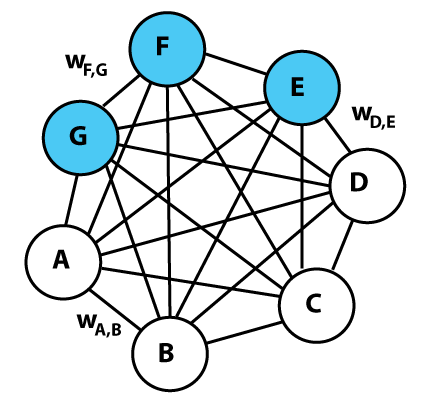
\includegraphics[width=0.4\linewidth]{{fig/bm}.png}
    \caption*{Structure of Boltzmann machine}
\end{figure}

A Boltzmann machine is a type of stochastic recurrent neural network that is known to be widely applied to binary model inference problems. By inspecting the above diagram, it is clear that the Boltzmann machine is different to the neurol network (or deep belief network, to be precise) as it:

\begin{itemize}
    \item Has no output layer and it is undirected.
    \item Has connections between input (in this case, the three blue) nodes.
\end{itemize}

The second property can be even more elaborate to the fact that every visible nodes within a Boltzmann machine can connect to each other, but this is merely a structure difference -- a restriced Boltzmann machine will not have this property, but still has no output nodes (and this will be a layer/block within deep neural network). The Boltzmann machine is an energy based system, where as each visible node will take a binary input, and by calculate the total energy of the system, we may infer on probablity of a particular visible node, or join distribution of couple visible nodes.

The energy of the total system is denoted as $E$, where:

\begin{equation*}
    -E(v, h) = \sum_{i \in v} v_i b_i + \sum_{k \in h} h_k b_k + \sum_{i \leq j} v_i v_j w_{ij} + \sum_{i, k} v_i h_k w_{ik} + \sum_{k \leq l} h_k h_l w_{kl}
\end{equation*}

\begin{itemize}
    \item $v$: visible nodes.
    \item $h$: hidden nodes.
    \item $b_i$: bias of node with index $i$, wheather this node is $v_i$ or $h_i$ is implied through mutiplication. i.e., $b_i$ in $h_i b_i$ is the bias of a hidden node $h_i$
    \item $w_{ij}$: weight between nodes of index $i$ and $j$, wheather the nodes are visible or not (or one visible one hidden) is implied through mutiplication.
\end{itemize}

Since the energy formula is quite long, it might be hard to digest. But essentially, take an edge of the proposed network (say it is $e$) and mutiply it with two of its verticies (say it is $e_A, e_B$), keep the result and sum it up by doing this to every edges as $\sum\limits_{e \in E(G)} e e_A e_B$. Here's an example made by \href{https://www.youtube.com/watch?v=5jaBneYd5Ig}{Colin Reckons} (note we omitted connection between visible nodes for simplicity):

\begin{figure}[H]
    \centering
    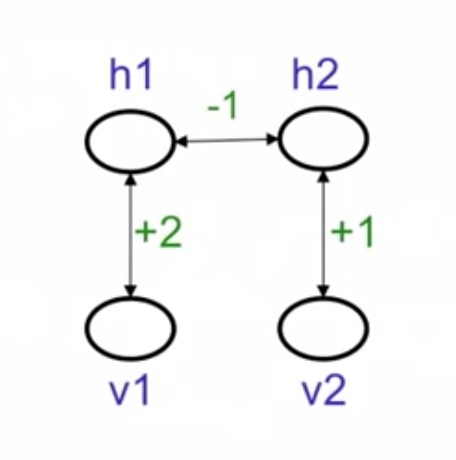
\includegraphics[width=0.3\linewidth]{{fig/bm_example}.png}
    \caption*{An example Boltzmann machine}
\end{figure}

Say we have $-E(<v_1, v_2, h_1, h_2>)$, the total energy of the network is:

\begin{align*}
    -E(<v_1, v_2, h_1, h_2>) &= w_{v_1 h_1}(v_1 \cdot h_1) - w_{h_1 h_2}(h_1 \cdot h_2) + w_{h_2 v_2}(h_2 \cdot v_2) =  2\\
    -E(<1, 1, 1, 1>) &= 2(1 \cdot 1) - 1(1 \cdot 1) + 1(1 \cdot 1) =  2\\
    -E(<1, 1, 1, 0>) &= 2(1 \cdot 1) + 1(1 \cdot 0) + 1(0 \cdot 1) = 2 \\
    &\dots
\end{align*}

We denote this total energy as $-E(v, h)$ to represent it is the total energy among all visible and hidden nodes; and we may infer the probablity of $p(v, h)$ and $p(v)$ as:

\begin{align*}
    p(v, h) &= \frac{e^{-E(v, h)}}{\sum_{u, g} e^{-E(u, g)}} \\
    p(v) &= \frac{\sum_h e^{-E(v, h)}}{\sum_{u, g} e^{-E(u, g)}}
\end{align*}

Where $u, g$ represents all possible combination of vissible and hidden nodes. In this example, we have $<v_1, h_2, h_1, h_2>$ to be a 4-bit binary vector, so there can be 16 possible combinations. Thus, we may proceed and infer the possible of all conditions as:

\begin{figure}[H]
    \centering
    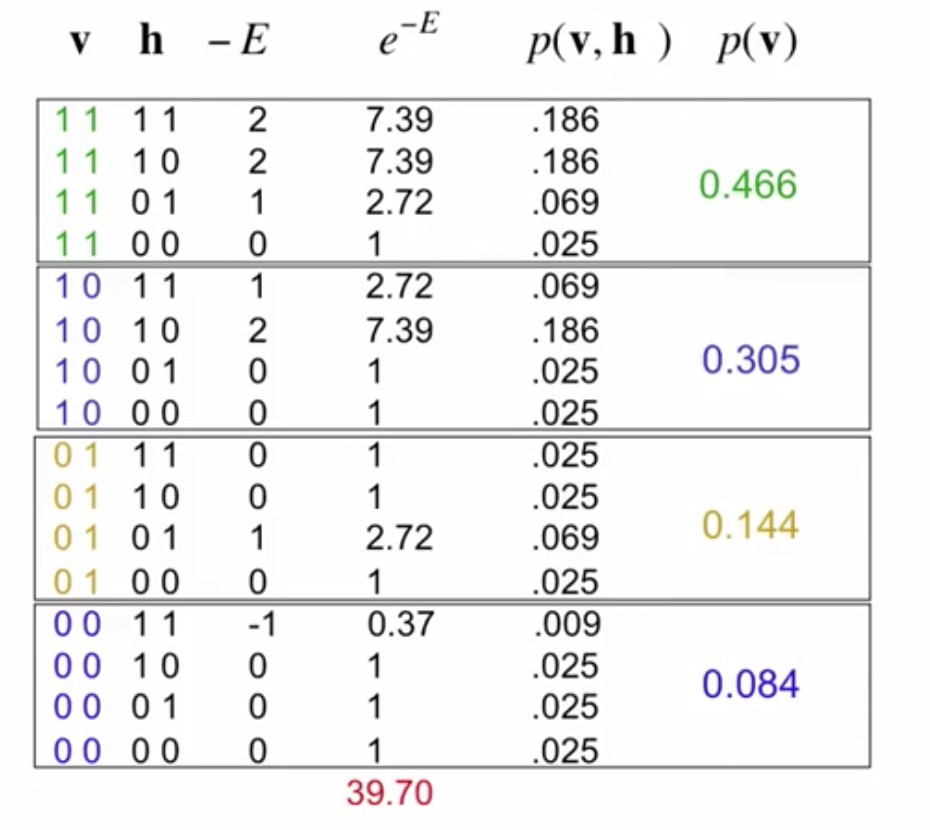
\includegraphics[width=0.7\linewidth]{{fig/bm_result}.png}
    \caption*{Probablity inferences of the example Boltzmann machine}
\end{figure}

Note this \textcolor{red}{39.70} is simply the sum of all $e^{-E}$, and each $p(v, h)$ are the $e^{-E}$ on its row divided by this 39.70. And the four $p(v)$ are sum of all $p(v, h)$ with the same $v$ inputs.\newline

\paragraph{Representation power on 2- and 3-unit binary input.}
Now we want to show that \textbf{ANY} distribution of a two-unit binary input (with excaption of having extreme output like $0, 1$, which requires a sum-of-weighted-inputs of $\pm infty$) can be represented by the Boltzmann machine and also a sigmoid feedforward network. We start with the sigmoid feedforward network.

\begin{figure}[H]
    \centering
    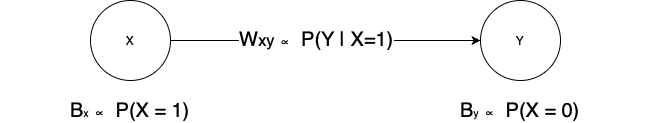
\includegraphics[width=0.7\linewidth]{{fig/2_unit}.png}
    \caption*{A Sigmoid feedforward network that can represent any distribution of a two-unit binary input.}
\end{figure}

It is easy to tell that this network can represent any distribution of a two-unit binary input, as we have $P(Y \mid X=1)$ and all possible $P(X)$s, all we have to do is to make it proportional to the sigmoid transformation so that $\sigma(z)$ can be the desired probablity output (where $z$ is the sum of weighted inputs). \newline

Now to represent the same distribution with a Boltzmann machine. We have the energy of $<0, 0>$ to be always zero, so the $p(<0, 0>)$ must relay on the its proportion to the sum of all energy. For $<1, 0>$ and $<0, 1>$, we may simply set the desired probablity distribution to be proportional to bias of each $1$ node, as the total energy in such state is always $e^{-B_x}$ (assuming $x$ is the node with $1$). Last, for the state $<1, 1>$, we may set the desired probablity to be proportional to the weight $w_{xy}$. As this Boltzmann machine can represent the distributions all four states of a 2 unit binary input with the same bias and weights, it can also represent any distribution of a two-unit binary input just like the sigmoid feedforward network.

This inference can be further elaborated to three-unit binary input as showned in \href{http://www.cs.toronto.edu/~bonner/courses/2016s/csc321/readings/Connectionist%20learning%20of%20belief%20networks.pdf}{R.M. Neal, Connectionist learning of belief networks, Artificial Intelligence 56 (1992) 71–113.} by doing what we did first for the first to node, and connect to third node with weights of its conditional probablity to the first two nodes. However, it can only be shown a distribution that is representable in sigmoid feedforward network is equally representable in a Boltzmann machine and vice versa. This is not to say that any \textbf{ANY} (non-extreme, as for no $0, 1$ probablity outputs) distribution of a three-unit binary input can be represent in a sigmoid feedforward network / Boltzmann machine, as in \textbf{Question 4.4.} we have shown a three-unit system with noisy-OR distribution can't be represented by a sigmoid feedforward network.

\paragraph{Representation power on 4-unit binary input.}

So far, although we have demonstrated that there are (non-extreme) distribution of 3-unit binary input that cannot be represented by a sigmoid network or a Boltzmann machine, the two still got the same representation power. But this is not the case when we raise to 4-unit binay input, as each of them got some distribution the other can't represent. Due to time and space constraint, here's a Boltzmann machine that can't be represent by a sigmoid netwrok, designed by R.M. Neal:


\begin{figure}[H]
    \centering
    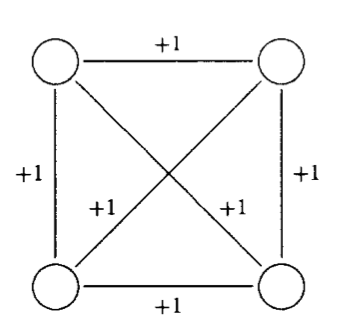
\includegraphics[width=0.3\linewidth]{{fig/bm_no_sig}.png}
    \caption*{A Boltzmann machine that is untranslatable to sigmoid belief network}
\end{figure}


Since the Boltzmann machine is symmetric, we mays start with any node and call this unit 4. For the weights that going into the second-last unit (unit 3 ), due to the symmetry shape, the two weights must be equal (we denote them as $w$, and let the bias of unit 3 to be $b$). Now in the case of unit 3 and unit 4 have value of 1s, and unit 1 and unit 2 have zero or one or two ones among them, we must have the following relationship (LHS Boltzmann and RHS sigmoid):

\begin{align*}
    e^{1} &= \propto e^b \frac{\sigma(1)}{\sigma{0}} &\text{zero 1 in unit 1\&2} \\
    e^{2} &= \propto e^{b + w} \frac{\sigma(2)}{\sigma{1}} &\text{one 1 in unit 1\&2} \\
    e^{3} &= \propto e^{b + 2w} \frac{\sigma(3)}{\sigma{2}} &\text{two 1s in unit 1\&2}
\end{align*}

Which is clear that this is not a solvable linear system, and therefore this distribution cannot be translate to a sigmoid belief network.




\end{document}

